% Options for packages loaded elsewhere
\PassOptionsToPackage{unicode}{hyperref}
\PassOptionsToPackage{hyphens}{url}
\PassOptionsToPackage{dvipsnames,svgnames,x11names}{xcolor}
%
\documentclass[
  letterpaper,
  DIV=11,
  numbers=noendperiod]{scrartcl}

\usepackage{amsmath,amssymb}
\usepackage{iftex}
\ifPDFTeX
  \usepackage[T1]{fontenc}
  \usepackage[utf8]{inputenc}
  \usepackage{textcomp} % provide euro and other symbols
\else % if luatex or xetex
  \usepackage{unicode-math}
  \defaultfontfeatures{Scale=MatchLowercase}
  \defaultfontfeatures[\rmfamily]{Ligatures=TeX,Scale=1}
\fi
\usepackage{lmodern}
\ifPDFTeX\else  
    % xetex/luatex font selection
\fi
% Use upquote if available, for straight quotes in verbatim environments
\IfFileExists{upquote.sty}{\usepackage{upquote}}{}
\IfFileExists{microtype.sty}{% use microtype if available
  \usepackage[]{microtype}
  \UseMicrotypeSet[protrusion]{basicmath} % disable protrusion for tt fonts
}{}
\makeatletter
\@ifundefined{KOMAClassName}{% if non-KOMA class
  \IfFileExists{parskip.sty}{%
    \usepackage{parskip}
  }{% else
    \setlength{\parindent}{0pt}
    \setlength{\parskip}{6pt plus 2pt minus 1pt}}
}{% if KOMA class
  \KOMAoptions{parskip=half}}
\makeatother
\usepackage{xcolor}
\setlength{\emergencystretch}{3em} % prevent overfull lines
\setcounter{secnumdepth}{-\maxdimen} % remove section numbering
% Make \paragraph and \subparagraph free-standing
\makeatletter
\ifx\paragraph\undefined\else
  \let\oldparagraph\paragraph
  \renewcommand{\paragraph}{
    \@ifstar
      \xxxParagraphStar
      \xxxParagraphNoStar
  }
  \newcommand{\xxxParagraphStar}[1]{\oldparagraph*{#1}\mbox{}}
  \newcommand{\xxxParagraphNoStar}[1]{\oldparagraph{#1}\mbox{}}
\fi
\ifx\subparagraph\undefined\else
  \let\oldsubparagraph\subparagraph
  \renewcommand{\subparagraph}{
    \@ifstar
      \xxxSubParagraphStar
      \xxxSubParagraphNoStar
  }
  \newcommand{\xxxSubParagraphStar}[1]{\oldsubparagraph*{#1}\mbox{}}
  \newcommand{\xxxSubParagraphNoStar}[1]{\oldsubparagraph{#1}\mbox{}}
\fi
\makeatother

\usepackage{color}
\usepackage{fancyvrb}
\newcommand{\VerbBar}{|}
\newcommand{\VERB}{\Verb[commandchars=\\\{\}]}
\DefineVerbatimEnvironment{Highlighting}{Verbatim}{commandchars=\\\{\}}
% Add ',fontsize=\small' for more characters per line
\usepackage{framed}
\definecolor{shadecolor}{RGB}{241,243,245}
\newenvironment{Shaded}{\begin{snugshade}}{\end{snugshade}}
\newcommand{\AlertTok}[1]{\textcolor[rgb]{0.68,0.00,0.00}{#1}}
\newcommand{\AnnotationTok}[1]{\textcolor[rgb]{0.37,0.37,0.37}{#1}}
\newcommand{\AttributeTok}[1]{\textcolor[rgb]{0.40,0.45,0.13}{#1}}
\newcommand{\BaseNTok}[1]{\textcolor[rgb]{0.68,0.00,0.00}{#1}}
\newcommand{\BuiltInTok}[1]{\textcolor[rgb]{0.00,0.23,0.31}{#1}}
\newcommand{\CharTok}[1]{\textcolor[rgb]{0.13,0.47,0.30}{#1}}
\newcommand{\CommentTok}[1]{\textcolor[rgb]{0.37,0.37,0.37}{#1}}
\newcommand{\CommentVarTok}[1]{\textcolor[rgb]{0.37,0.37,0.37}{\textit{#1}}}
\newcommand{\ConstantTok}[1]{\textcolor[rgb]{0.56,0.35,0.01}{#1}}
\newcommand{\ControlFlowTok}[1]{\textcolor[rgb]{0.00,0.23,0.31}{\textbf{#1}}}
\newcommand{\DataTypeTok}[1]{\textcolor[rgb]{0.68,0.00,0.00}{#1}}
\newcommand{\DecValTok}[1]{\textcolor[rgb]{0.68,0.00,0.00}{#1}}
\newcommand{\DocumentationTok}[1]{\textcolor[rgb]{0.37,0.37,0.37}{\textit{#1}}}
\newcommand{\ErrorTok}[1]{\textcolor[rgb]{0.68,0.00,0.00}{#1}}
\newcommand{\ExtensionTok}[1]{\textcolor[rgb]{0.00,0.23,0.31}{#1}}
\newcommand{\FloatTok}[1]{\textcolor[rgb]{0.68,0.00,0.00}{#1}}
\newcommand{\FunctionTok}[1]{\textcolor[rgb]{0.28,0.35,0.67}{#1}}
\newcommand{\ImportTok}[1]{\textcolor[rgb]{0.00,0.46,0.62}{#1}}
\newcommand{\InformationTok}[1]{\textcolor[rgb]{0.37,0.37,0.37}{#1}}
\newcommand{\KeywordTok}[1]{\textcolor[rgb]{0.00,0.23,0.31}{\textbf{#1}}}
\newcommand{\NormalTok}[1]{\textcolor[rgb]{0.00,0.23,0.31}{#1}}
\newcommand{\OperatorTok}[1]{\textcolor[rgb]{0.37,0.37,0.37}{#1}}
\newcommand{\OtherTok}[1]{\textcolor[rgb]{0.00,0.23,0.31}{#1}}
\newcommand{\PreprocessorTok}[1]{\textcolor[rgb]{0.68,0.00,0.00}{#1}}
\newcommand{\RegionMarkerTok}[1]{\textcolor[rgb]{0.00,0.23,0.31}{#1}}
\newcommand{\SpecialCharTok}[1]{\textcolor[rgb]{0.37,0.37,0.37}{#1}}
\newcommand{\SpecialStringTok}[1]{\textcolor[rgb]{0.13,0.47,0.30}{#1}}
\newcommand{\StringTok}[1]{\textcolor[rgb]{0.13,0.47,0.30}{#1}}
\newcommand{\VariableTok}[1]{\textcolor[rgb]{0.07,0.07,0.07}{#1}}
\newcommand{\VerbatimStringTok}[1]{\textcolor[rgb]{0.13,0.47,0.30}{#1}}
\newcommand{\WarningTok}[1]{\textcolor[rgb]{0.37,0.37,0.37}{\textit{#1}}}

\providecommand{\tightlist}{%
  \setlength{\itemsep}{0pt}\setlength{\parskip}{0pt}}\usepackage{longtable,booktabs,array}
\usepackage{calc} % for calculating minipage widths
% Correct order of tables after \paragraph or \subparagraph
\usepackage{etoolbox}
\makeatletter
\patchcmd\longtable{\par}{\if@noskipsec\mbox{}\fi\par}{}{}
\makeatother
% Allow footnotes in longtable head/foot
\IfFileExists{footnotehyper.sty}{\usepackage{footnotehyper}}{\usepackage{footnote}}
\makesavenoteenv{longtable}
\usepackage{graphicx}
\makeatletter
\def\maxwidth{\ifdim\Gin@nat@width>\linewidth\linewidth\else\Gin@nat@width\fi}
\def\maxheight{\ifdim\Gin@nat@height>\textheight\textheight\else\Gin@nat@height\fi}
\makeatother
% Scale images if necessary, so that they will not overflow the page
% margins by default, and it is still possible to overwrite the defaults
% using explicit options in \includegraphics[width, height, ...]{}
\setkeys{Gin}{width=\maxwidth,height=\maxheight,keepaspectratio}
% Set default figure placement to htbp
\makeatletter
\def\fps@figure{htbp}
\makeatother

\usepackage{float}
\usepackage{tabularray}
\usepackage[normalem]{ulem}
\usepackage{graphicx}
\UseTblrLibrary{booktabs}
\UseTblrLibrary{rotating}
\UseTblrLibrary{siunitx}
\NewTableCommand{\tinytableDefineColor}[3]{\definecolor{#1}{#2}{#3}}
\newcommand{\tinytableTabularrayUnderline}[1]{\underline{#1}}
\newcommand{\tinytableTabularrayStrikeout}[1]{\sout{#1}}
\usepackage{booktabs}
\usepackage{caption}
\usepackage{longtable}
\usepackage{colortbl}
\usepackage{array}
\usepackage{anyfontsize}
\usepackage{multirow}
\KOMAoption{captions}{tableheading}
\makeatletter
\@ifpackageloaded{caption}{}{\usepackage{caption}}
\AtBeginDocument{%
\ifdefined\contentsname
  \renewcommand*\contentsname{Table of contents}
\else
  \newcommand\contentsname{Table of contents}
\fi
\ifdefined\listfigurename
  \renewcommand*\listfigurename{List of Figures}
\else
  \newcommand\listfigurename{List of Figures}
\fi
\ifdefined\listtablename
  \renewcommand*\listtablename{List of Tables}
\else
  \newcommand\listtablename{List of Tables}
\fi
\ifdefined\figurename
  \renewcommand*\figurename{Figure}
\else
  \newcommand\figurename{Figure}
\fi
\ifdefined\tablename
  \renewcommand*\tablename{Table}
\else
  \newcommand\tablename{Table}
\fi
}
\@ifpackageloaded{float}{}{\usepackage{float}}
\floatstyle{ruled}
\@ifundefined{c@chapter}{\newfloat{codelisting}{h}{lop}}{\newfloat{codelisting}{h}{lop}[chapter]}
\floatname{codelisting}{Listing}
\newcommand*\listoflistings{\listof{codelisting}{List of Listings}}
\makeatother
\makeatletter
\makeatother
\makeatletter
\@ifpackageloaded{caption}{}{\usepackage{caption}}
\@ifpackageloaded{subcaption}{}{\usepackage{subcaption}}
\makeatother

\ifLuaTeX
  \usepackage{selnolig}  % disable illegal ligatures
\fi
\usepackage{bookmark}

\IfFileExists{xurl.sty}{\usepackage{xurl}}{} % add URL line breaks if available
\urlstyle{same} % disable monospaced font for URLs
\hypersetup{
  pdftitle={Lesson 1},
  colorlinks=true,
  linkcolor={blue},
  filecolor={Maroon},
  citecolor={Blue},
  urlcolor={Blue},
  pdfcreator={LaTeX via pandoc}}


\title{Lesson 1}
\usepackage{etoolbox}
\makeatletter
\providecommand{\subtitle}[1]{% add subtitle to \maketitle
  \apptocmd{\@title}{\par {\large #1 \par}}{}{}
}
\makeatother
\subtitle{Introduction to forecast modelling}
\author{}
\date{}

\begin{document}
\maketitle


\subsection{Exercises - Bias in Self-reported
Turnout}\label{exercises---bias-in-self-reported-turnout}

Surveys are frequently used to measure political behavior such as voter
turnout, but some researchers are concerned about the accuracy of
self-reports. In particular, they worry about possible social
desirability bias where in post-election surveys, respondents who did
not vote in an election lie about not having voted because they may feel
that they should have voted. Is such a bias present in the American
National Election Studies (ANES)? The ANES is a nation- wide survey that
has been conducted for every election since 1948. The ANES conducts
face-to-face interviews with a nationally representative sample of
adults. The table below displays the names and descriptions of variables
in the turnout.csv data file.

First we load all the necessary packages.

\begin{Shaded}
\begin{Highlighting}[]
\FunctionTok{library}\NormalTok{(tidyverse)}
\FunctionTok{library}\NormalTok{(modelsummary)}
\FunctionTok{library}\NormalTok{(tinytable)}
\FunctionTok{library}\NormalTok{(gtsummary)}
\end{Highlighting}
\end{Shaded}

\subsubsection{Question 1}\label{question-1}

Load the data into R and check the dimensions of the data. Also, obtain
a summary of the data. How many observations are there? What is the
range of years covered in this data set?

\begin{Shaded}
\begin{Highlighting}[]
\ControlFlowTok{if}\NormalTok{ (}\FunctionTok{interactive}\NormalTok{()) \{}
\NormalTok{  turnout\_file }\OtherTok{\textless{}{-}} \StringTok{"../1 {-} Introduction {-} Forecast Modeling/turnout.csv"}
\NormalTok{\} }\ControlFlowTok{else}\NormalTok{ \{}
\NormalTok{  turnout\_file }\OtherTok{\textless{}{-}} \StringTok{"../../1 {-} Introduction {-} Forecast Modeling/turnout.csv"}
\NormalTok{\}}

\NormalTok{turnout }\OtherTok{\textless{}{-}} \FunctionTok{read.csv}\NormalTok{(turnout\_file)}

\NormalTok{dims }\OtherTok{\textless{}{-}} \FunctionTok{dim}\NormalTok{(turnout)}
\NormalTok{obs }\OtherTok{\textless{}{-}} \FunctionTok{nrow}\NormalTok{(turnout)}
\NormalTok{years }\OtherTok{\textless{}{-}} \FunctionTok{range}\NormalTok{(turnout}\SpecialCharTok{$}\NormalTok{year)}
\end{Highlighting}
\end{Shaded}

In this dataset there is 14 observations. The dimensions are 14 by 9 and
the year-range is from 1980 to 2008.

\begin{Shaded}
\begin{Highlighting}[]
\FunctionTok{head}\NormalTok{(turnout)}
\end{Highlighting}
\end{Shaded}

\begin{verbatim}
  year    VEP    VAP total ANES felons noncit overseas osvoters
1 1980 159635 164445 86515   71    802   5756     1803       NA
2 1982 160467 166028 67616   60    960   6641     1982       NA
3 1984 167702 173995 92653   74   1165   7482     2361       NA
4 1986 170396 177922 64991   53   1367   8362     2216       NA
5 1988 173579 181955 91595   70   1594   9280     2257       NA
6 1990 176629 186159 67859   47   1901  10239     2659       NA
\end{verbatim}

\subsubsection{Question 2}\label{question-2}

Calculate the turnout rate based on the voting age population or VAP.
Note that for this data set, we must add the total number of eligible
overseas voters since the VAP variable does not include these
individuals in the count. Next, calculate the turnout rate using the
voting eligible population or VEP. What difference do you observe?

\begin{Shaded}
\begin{Highlighting}[]
\NormalTok{turnout }\OtherTok{\textless{}{-}}\NormalTok{ turnout }\SpecialCharTok{\%\textgreater{}\%} 
  \FunctionTok{select}\NormalTok{(}\FunctionTok{everything}\NormalTok{()) }\SpecialCharTok{\%\textgreater{}\%} 
  \FunctionTok{mutate}\NormalTok{(}\AttributeTok{vap\_os =}\NormalTok{ VAP }\SpecialCharTok{+} \FunctionTok{na.omit}\NormalTok{(overseas),}
         \AttributeTok{turnout\_rate\_vap =}\NormalTok{ (total }\SpecialCharTok{/}\NormalTok{ vap\_os) }\SpecialCharTok{*} \DecValTok{100}\NormalTok{,}
         \AttributeTok{turnout\_rate\_vep =}\NormalTok{ (total }\SpecialCharTok{/}\NormalTok{ VEP) }\SpecialCharTok{*} \DecValTok{100}\NormalTok{,}
         \AttributeTok{turnout\_rate\_diff =}\NormalTok{ turnout\_rate\_vep }\SpecialCharTok{{-}}\NormalTok{ turnout\_rate\_vap,}
         \AttributeTok{election\_type =} \FunctionTok{if\_else}\NormalTok{(year }\SpecialCharTok{/} \DecValTok{4} \SpecialCharTok{==} \FunctionTok{round}\NormalTok{(year }\SpecialCharTok{/} \DecValTok{4}\NormalTok{),}
                                 \StringTok{"presidential"}\NormalTok{, }\StringTok{"midterm"}\NormalTok{),}
         \AttributeTok{year =} \FunctionTok{as\_factor}\NormalTok{(year))}
\NormalTok{turnout }\SpecialCharTok{\%\textgreater{}\%} 
  \FunctionTok{select}\NormalTok{(}\FunctionTok{starts\_with}\NormalTok{(}\StringTok{"turnout\_rate"}\NormalTok{)) }\SpecialCharTok{\%\textgreater{}\%} 
  \FunctionTok{mutate}\NormalTok{(}\StringTok{\textquotesingle{}VAP \%\textquotesingle{}} \OtherTok{=}\NormalTok{ turnout\_rate\_vap,}
         \StringTok{\textquotesingle{}VEP \%\textquotesingle{}} \OtherTok{=}\NormalTok{ turnout\_rate\_vep,}
         \AttributeTok{DIFF =}\NormalTok{ turnout\_rate\_diff) }\SpecialCharTok{\%\textgreater{}\%} 
  \FunctionTok{select}\NormalTok{(}\SpecialCharTok{{-}}\FunctionTok{starts\_with}\NormalTok{(}\StringTok{"turnout\_rate"}\NormalTok{)) }\SpecialCharTok{\%\textgreater{}\%} 
  \FunctionTok{datasummary\_skim}\NormalTok{(}\AttributeTok{fmt =} \DecValTok{3}\NormalTok{,}
                   \AttributeTok{fun\_numeric =} \FunctionTok{list}\NormalTok{(}
                     \StringTok{\textquotesingle{}n(years)\textquotesingle{}} \OtherTok{=}\NormalTok{ NUnique,}
                     \AttributeTok{Mean =}\NormalTok{ Mean,}
                     \AttributeTok{SD =}\NormalTok{ SD,}
                     \AttributeTok{Min =}\NormalTok{ Min,}
                     \CommentTok{\# Median = Median,}
                     \AttributeTok{Max =}\NormalTok{ Max,}
                     \AttributeTok{Histogram =} \ControlFlowTok{function}\NormalTok{(x) }\StringTok{""}\NormalTok{))}
\end{Highlighting}
\end{Shaded}

\begin{table}
\centering
\begin{tblr}[         %% tabularray outer open
]                     %% tabularray outer close
{                     %% tabularray inner open
colspec={Q[]Q[]Q[]Q[]Q[]Q[]Q[]},
column{1}={halign=l,},
column{2}={halign=l,},
column{3}={halign=l,},
column{4}={halign=l,},
column{5}={halign=l,},
column{6}={halign=l,},
column{7}={halign=l,},
}                     %% tabularray inner close
\toprule
& n(years) & Mean & SD & Min & Max & Histogram \\ \midrule %% TinyTableHeader
VAP \% & 14 & 45.457 & 8.125 & 34.832 & 55.674 & 
\includegraphics[height=1em]{tinytable_assets/idzkve95a6m70npyx6c2fy.png} \\
VEP \% & 14 & 48.949 & 8.886 & 38.093 & 61.554 & 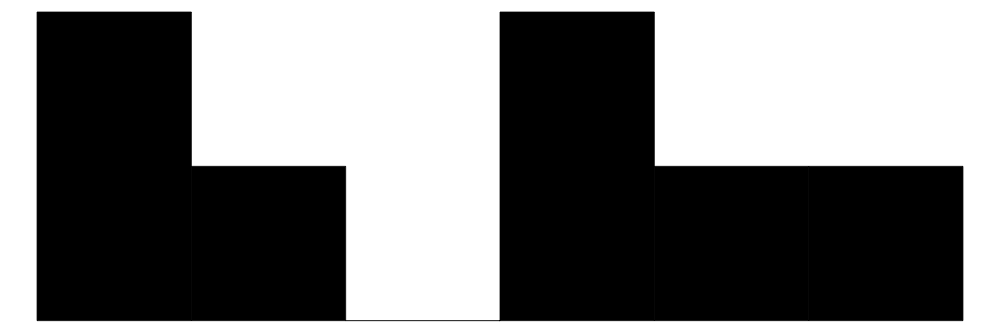
\includegraphics[height=1em]{tinytable_assets/id7l1au4bvl5mqar4qbnv0.png} \\
DIFF & 14 & 3.493 & 1.274 & 1.892 & 5.880 & 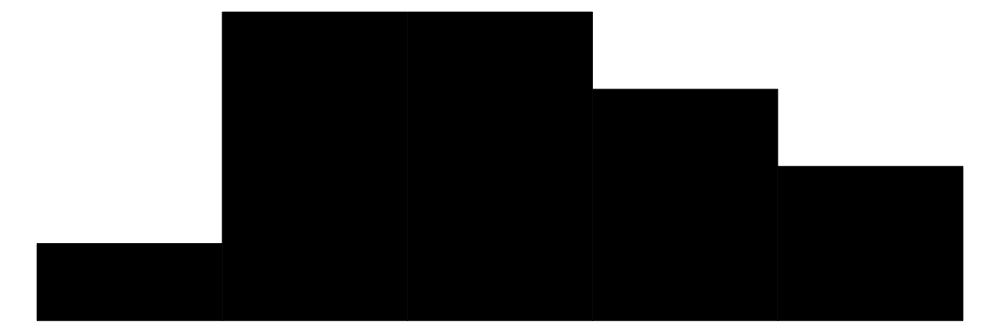
\includegraphics[height=1em]{tinytable_assets/idvsd4ys4x4hh29f620hva.png} \\
\bottomrule
\end{tblr}
\end{table}

\begin{Shaded}
\begin{Highlighting}[]
\NormalTok{turnout }\SpecialCharTok{\%\textgreater{}\%} 
  \FunctionTok{ggplot}\NormalTok{() }\SpecialCharTok{+}
  \FunctionTok{geom\_point}\NormalTok{(}\FunctionTok{aes}\NormalTok{(}\AttributeTok{x =}\NormalTok{ year, }\AttributeTok{y =}\NormalTok{ turnout\_rate\_vap, }\AttributeTok{shape =}\NormalTok{ election\_type, }\AttributeTok{color =}\NormalTok{ election\_type)) }\SpecialCharTok{+}
  \FunctionTok{geom\_line}\NormalTok{(}\FunctionTok{aes}\NormalTok{(}\AttributeTok{x =}\NormalTok{ year, }\AttributeTok{y =}\NormalTok{ turnout\_rate\_vap, }\AttributeTok{group =} \DecValTok{1}\NormalTok{), }\AttributeTok{color =} \StringTok{"lightblue"}\NormalTok{) }\SpecialCharTok{+}
  \FunctionTok{geom\_point}\NormalTok{(}\FunctionTok{aes}\NormalTok{(}\AttributeTok{x =}\NormalTok{ year, }\AttributeTok{y =}\NormalTok{ turnout\_rate\_vep, }\AttributeTok{shape =}\NormalTok{ election\_type, }\AttributeTok{color =}\NormalTok{ election\_type)) }\SpecialCharTok{+}
  \FunctionTok{geom\_line}\NormalTok{(}\FunctionTok{aes}\NormalTok{(}\AttributeTok{x =}\NormalTok{ year, }\AttributeTok{y =}\NormalTok{ turnout\_rate\_vep, }\AttributeTok{group =} \DecValTok{1}\NormalTok{), }\AttributeTok{color =} \StringTok{"lightgreen"}\NormalTok{) }\SpecialCharTok{+}
  \FunctionTok{theme\_minimal}\NormalTok{()}
\end{Highlighting}
\end{Shaded}

\begin{center}
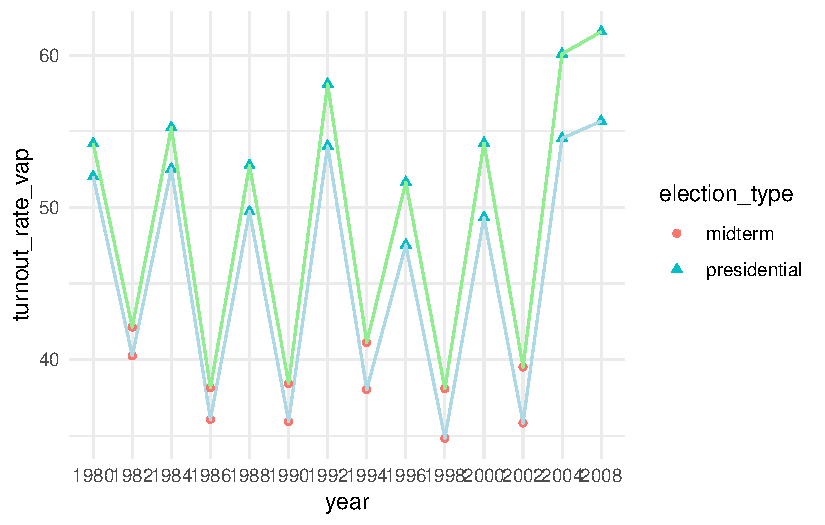
\includegraphics{class-1_files/figure-pdf/unnamed-chunk-4-1.pdf}
\end{center}

The Voting Eligible Population (green) generally has a higher turnout
rate than the Voting Age Population. It is on average 3.493. There is
also generally higher turnout for the presidential elections than there
are for the midterms.

\subsubsection{Question 3}\label{question-3}

Compute the difference between VAP and ANES estimates of turnout rate.
How big is the difference on average? What is the range of the
difference? Conduct the same comparison for the VEP and ANES estimates
of voter turnout. Briefly comment on the results.

\begin{Shaded}
\begin{Highlighting}[]
\NormalTok{turnout }\OtherTok{\textless{}{-}}\NormalTok{ turnout }\SpecialCharTok{\%\textgreater{}\%} 
  \FunctionTok{select}\NormalTok{(}\FunctionTok{everything}\NormalTok{()) }\SpecialCharTok{\%\textgreater{}\%} 
  \FunctionTok{mutate}\NormalTok{(}\AttributeTok{vap\_anes =}\NormalTok{ ANES }\SpecialCharTok{{-}}\NormalTok{ turnout\_rate\_vap,}
         \AttributeTok{vep\_anes =}\NormalTok{ ANES }\SpecialCharTok{{-}}\NormalTok{ turnout\_rate\_vep)}
\NormalTok{turnout }\SpecialCharTok{\%\textgreater{}\%} 
  \FunctionTok{select}\NormalTok{(}\FunctionTok{ends\_with}\NormalTok{(}\StringTok{"\_anes"}\NormalTok{)) }\SpecialCharTok{\%\textgreater{}\%} 
  \FunctionTok{mutate}\NormalTok{(}\StringTok{\textquotesingle{}ANES {-} VAP\textquotesingle{}} \OtherTok{=}\NormalTok{ vap\_anes,}
         \StringTok{\textquotesingle{}ANES {-} VEP\textquotesingle{}} \OtherTok{=}\NormalTok{ vep\_anes) }\SpecialCharTok{\%\textgreater{}\%} 
  \FunctionTok{select}\NormalTok{(}\SpecialCharTok{!}\FunctionTok{ends\_with}\NormalTok{(}\StringTok{"\_anes"}\NormalTok{)) }\SpecialCharTok{\%\textgreater{}\%} 
  \FunctionTok{datasummary\_skim}\NormalTok{(}\AttributeTok{fmt =} \DecValTok{3}\NormalTok{,}
                   \AttributeTok{fun\_numeric =} \FunctionTok{list}\NormalTok{(}
                     \StringTok{\textquotesingle{}n(years)\textquotesingle{}} \OtherTok{=}\NormalTok{ NUnique,}
                     \AttributeTok{Mean =}\NormalTok{ Mean,}
                     \AttributeTok{SD =}\NormalTok{ SD,}
                     \AttributeTok{Min =}\NormalTok{ Min,}
                     \CommentTok{\# Median = Median,}
                     \AttributeTok{Max =}\NormalTok{ Max,}
                     \AttributeTok{Histogram =} \ControlFlowTok{function}\NormalTok{(x) }\StringTok{""}\NormalTok{))}
\end{Highlighting}
\end{Shaded}

\begin{table}
\centering
\begin{tblr}[         %% tabularray outer open
]                     %% tabularray outer close
{                     %% tabularray inner open
colspec={Q[]Q[]Q[]Q[]Q[]Q[]Q[]},
column{1}={halign=l,},
column{2}={halign=l,},
column{3}={halign=l,},
column{4}={halign=l,},
column{5}={halign=l,},
column{6}={halign=l,},
column{7}={halign=l,},
}                     %% tabularray inner close
\toprule
& n(years) & Mean & SD & Min & Max & Histogram \\ \midrule %% TinyTableHeader
ANES - VAP & 14 & 20.329 & 3.893 & 11.061 & 26.172 & 
\includegraphics[height=1em]{tinytable_assets/idqwr0bfhohc5vf9gghlkv.png} \\
ANES - VEP & 14 & 16.836 & 3.346 & 8.581 & 22.489 & 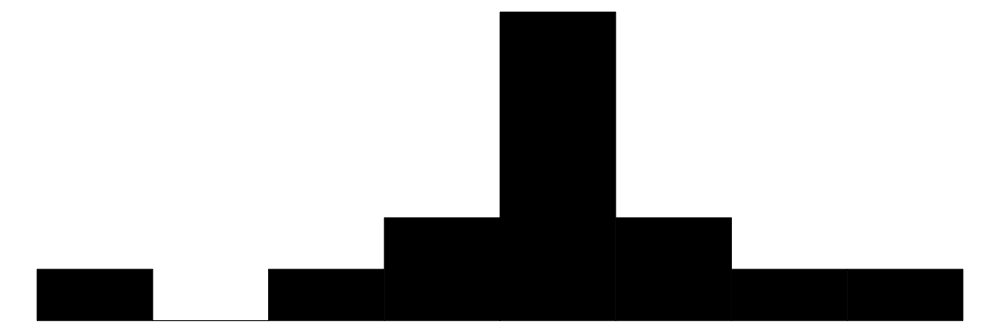
\includegraphics[height=1em]{tinytable_assets/idnvk2wljyp3sg9zd5o1v0.png} \\
\bottomrule
\end{tblr}
\end{table}

ANES is on average 20.3 points off of the actual VAP turnout. This is
not very convincing. In the same manner, ANES is on average 16.8 points
off of the actual VEP turnout.

\subsubsection{Question 4}\label{question-4}

Compare the VEP turnout rate with the ANES turnout rate separately for
presidential elections and midterm elections. Note that the data set
excludes the year 2006. Does the bias of the ANES vary across election
types?

\begin{itemize}
\tightlist
\item
  I have already decided which the types of elections in \emph{Question
  2}.
\end{itemize}

\begin{Shaded}
\begin{Highlighting}[]
\NormalTok{turnout }\SpecialCharTok{\%\textgreater{}\%} 
  \FunctionTok{select}\NormalTok{(turnout\_rate\_vep, ANES, vep\_anes, election\_type) }\SpecialCharTok{\%\textgreater{}\%} 
\NormalTok{  gtsummary}\SpecialCharTok{::}\FunctionTok{tbl\_summary}\NormalTok{(}\AttributeTok{by =} \StringTok{"election\_type"}\NormalTok{,}
                         \AttributeTok{label =} \FunctionTok{list}\NormalTok{(}
                           \AttributeTok{turnout\_rate\_vep =} \StringTok{"Voting Eligible Population"}\NormalTok{,}
                           \AttributeTok{ANES =} \StringTok{"ANES estimate"}\NormalTok{,}
                           \AttributeTok{vep\_anes =} \StringTok{"Differences between estimates"}
\NormalTok{                         ),}
                         \AttributeTok{statistic =} \FunctionTok{list}\NormalTok{(}\FunctionTok{all\_continuous}\NormalTok{() }\SpecialCharTok{\textasciitilde{}} \StringTok{"\{mean\} (\{min\} {-} \{max\})"}\NormalTok{))}
\end{Highlighting}
\end{Shaded}

\begingroup
\fontsize{12.0pt}{14.4pt}\selectfont
\setlength{\LTpost}{0mm}
\begin{longtable*}{lcc}
\toprule
\textbf{Characteristic} & \textbf{midterm}  N = 6\textsuperscript{\textit{1}} & \textbf{presidential}  N = 8\textsuperscript{\textit{1}} \\ 
\midrule\addlinespace[2.5pt]
Voting Eligible Population & 40 (38 - 42) & 56 (52 - 62) \\ 
ANES estimate & 55 (47 - 62) & 74 (70 - 78) \\ 
Differences between estimates & 15.43 (8.58 - 22.49) & 17.89 (16.45 - 21.34) \\ 
\bottomrule
\end{longtable*}
\begin{minipage}{\linewidth}
\textsuperscript{\textit{1}}Mean (Min - Max)\\
\end{minipage}
\endgroup

\begin{Shaded}
\begin{Highlighting}[]
\NormalTok{pct\_pres }\OtherTok{\textless{}{-}}\NormalTok{ turnout }\SpecialCharTok{\%\textgreater{}\%} 
  \FunctionTok{select}\NormalTok{(turnout\_rate\_vep, ANES, election\_type) }\SpecialCharTok{\%\textgreater{}\%} 
  \FunctionTok{mutate}\NormalTok{(}\AttributeTok{pct\_diff =}\NormalTok{ ANES }\SpecialCharTok{/}\NormalTok{ turnout\_rate\_vep) }\SpecialCharTok{\%\textgreater{}\%} 
  \FunctionTok{filter}\NormalTok{(election\_type }\SpecialCharTok{==} \StringTok{"presidential"}\NormalTok{) }\SpecialCharTok{\%\textgreater{}\%} 
  \FunctionTok{pull}\NormalTok{(pct\_diff) }\SpecialCharTok{\%\textgreater{}\%} 
  \FunctionTok{mean}\NormalTok{()}

\NormalTok{pct\_midterm }\OtherTok{\textless{}{-}}\NormalTok{ turnout }\SpecialCharTok{\%\textgreater{}\%} 
  \FunctionTok{select}\NormalTok{(turnout\_rate\_vep, ANES, election\_type) }\SpecialCharTok{\%\textgreater{}\%} 
  \FunctionTok{mutate}\NormalTok{(}\AttributeTok{pct\_diff =}\NormalTok{ ANES }\SpecialCharTok{/}\NormalTok{ turnout\_rate\_vep) }\SpecialCharTok{\%\textgreater{}\%} 
  \FunctionTok{filter}\NormalTok{(election\_type }\SpecialCharTok{==} \StringTok{"midterm"}\NormalTok{) }\SpecialCharTok{\%\textgreater{}\%} 
  \FunctionTok{pull}\NormalTok{(pct\_diff) }\SpecialCharTok{\%\textgreater{}\%} 
  \FunctionTok{mean}\NormalTok{()}

\NormalTok{pct\_diff }\OtherTok{\textless{}{-}}\NormalTok{ pct\_midterm }\SpecialCharTok{{-}}\NormalTok{ pct\_pres}

\NormalTok{pct }\OtherTok{\textless{}{-}} \FunctionTok{sapply}\NormalTok{(}\FunctionTok{list}\NormalTok{(pct\_pres, pct\_midterm, pct\_diff), round, }\DecValTok{3}\NormalTok{)}
\end{Highlighting}
\end{Shaded}

\begin{itemize}
\tightlist
\item
  It seems that the bias is a little larger when looking at the
  presidential elections. Then again, if expressed in percentages it is
  1.322 for presidential elections and 1.389 for midterms. In my
  interpretation, at least, the difference of 0.067 is close to
  nonsubstantial.
\end{itemize}

\subsubsection{Question 5}\label{question-5}

Divide the data into half by election years such that you subset the
data into two periods. Calculate the difference between the VEP turnout
rate and the ANES turnout rate separately for each period. Has the bias
of the ANES increased over time?

\begin{Shaded}
\begin{Highlighting}[]
\NormalTok{until\_1992 }\OtherTok{\textless{}{-}}\NormalTok{ turnout[}\DecValTok{1}\SpecialCharTok{:}\DecValTok{7}\NormalTok{,]}

\NormalTok{pct\_pres\_until }\OtherTok{\textless{}{-}}\NormalTok{ until\_1992 }\SpecialCharTok{\%\textgreater{}\%} 
  \FunctionTok{select}\NormalTok{(turnout\_rate\_vep, ANES, election\_type) }\SpecialCharTok{\%\textgreater{}\%} 
  \FunctionTok{mutate}\NormalTok{(}\AttributeTok{pct\_diff =}\NormalTok{ ANES }\SpecialCharTok{/}\NormalTok{ turnout\_rate\_vep) }\SpecialCharTok{\%\textgreater{}\%} 
  \FunctionTok{filter}\NormalTok{(election\_type }\SpecialCharTok{==} \StringTok{"presidential"}\NormalTok{) }\SpecialCharTok{\%\textgreater{}\%} 
  \FunctionTok{pull}\NormalTok{(pct\_diff) }\SpecialCharTok{\%\textgreater{}\%} 
  \FunctionTok{mean}\NormalTok{()}

\NormalTok{pct\_midterm\_until }\OtherTok{\textless{}{-}}\NormalTok{ until\_1992 }\SpecialCharTok{\%\textgreater{}\%} 
  \FunctionTok{select}\NormalTok{(turnout\_rate\_vep, ANES, election\_type) }\SpecialCharTok{\%\textgreater{}\%} 
  \FunctionTok{mutate}\NormalTok{(}\AttributeTok{pct\_diff =}\NormalTok{ ANES }\SpecialCharTok{/}\NormalTok{ turnout\_rate\_vep) }\SpecialCharTok{\%\textgreater{}\%} 
  \FunctionTok{filter}\NormalTok{(election\_type }\SpecialCharTok{==} \StringTok{"midterm"}\NormalTok{) }\SpecialCharTok{\%\textgreater{}\%} 
  \FunctionTok{pull}\NormalTok{(pct\_diff) }\SpecialCharTok{\%\textgreater{}\%} 
  \FunctionTok{mean}\NormalTok{()}

\NormalTok{pct\_diff\_until }\OtherTok{\textless{}{-}}\NormalTok{ pct\_midterm\_until }\SpecialCharTok{{-}}\NormalTok{ pct\_pres\_until}

\NormalTok{pct\_until }\OtherTok{\textless{}{-}} \FunctionTok{sapply}\NormalTok{(}\FunctionTok{list}\NormalTok{(pct\_pres\_until, pct\_midterm\_until, pct\_diff\_until), round, }\DecValTok{3}\NormalTok{)}
\end{Highlighting}
\end{Shaded}

\begin{Shaded}
\begin{Highlighting}[]
\NormalTok{after\_1992 }\OtherTok{\textless{}{-}}\NormalTok{ turnout[}\SpecialCharTok{{-}}\NormalTok{(}\DecValTok{1}\SpecialCharTok{:}\DecValTok{7}\NormalTok{),]}

\NormalTok{pct\_pres\_after }\OtherTok{\textless{}{-}}\NormalTok{ after\_1992 }\SpecialCharTok{\%\textgreater{}\%} 
  \FunctionTok{select}\NormalTok{(turnout\_rate\_vep, ANES, election\_type) }\SpecialCharTok{\%\textgreater{}\%} 
  \FunctionTok{mutate}\NormalTok{(}\AttributeTok{pct\_diff =}\NormalTok{ ANES }\SpecialCharTok{/}\NormalTok{ turnout\_rate\_vep) }\SpecialCharTok{\%\textgreater{}\%} 
  \FunctionTok{filter}\NormalTok{(election\_type }\SpecialCharTok{==} \StringTok{"presidential"}\NormalTok{) }\SpecialCharTok{\%\textgreater{}\%} 
  \FunctionTok{pull}\NormalTok{(pct\_diff) }\SpecialCharTok{\%\textgreater{}\%} 
  \FunctionTok{mean}\NormalTok{()}

\NormalTok{pct\_midterm\_after }\OtherTok{\textless{}{-}}\NormalTok{ after\_1992 }\SpecialCharTok{\%\textgreater{}\%} 
  \FunctionTok{select}\NormalTok{(turnout\_rate\_vep, ANES, election\_type) }\SpecialCharTok{\%\textgreater{}\%} 
  \FunctionTok{mutate}\NormalTok{(}\AttributeTok{pct\_diff =}\NormalTok{ ANES }\SpecialCharTok{/}\NormalTok{ turnout\_rate\_vep) }\SpecialCharTok{\%\textgreater{}\%} 
  \FunctionTok{filter}\NormalTok{(election\_type }\SpecialCharTok{==} \StringTok{"midterm"}\NormalTok{) }\SpecialCharTok{\%\textgreater{}\%} 
  \FunctionTok{pull}\NormalTok{(pct\_diff) }\SpecialCharTok{\%\textgreater{}\%} 
  \FunctionTok{mean}\NormalTok{()}

\NormalTok{pct\_diff\_after }\OtherTok{\textless{}{-}}\NormalTok{ pct\_midterm\_after }\SpecialCharTok{{-}}\NormalTok{ pct\_pres\_after}

\NormalTok{pct\_after }\OtherTok{\textless{}{-}} \FunctionTok{sapply}\NormalTok{(}\FunctionTok{list}\NormalTok{(pct\_pres\_after, pct\_midterm\_after, pct\_diff\_after), round, }\DecValTok{3}\NormalTok{)}
\end{Highlighting}
\end{Shaded}

Then we can compare the before and after

\begin{Shaded}
\begin{Highlighting}[]
\NormalTok{result }\OtherTok{\textless{}{-}}\NormalTok{ pct\_after }\SpecialCharTok{{-}}\NormalTok{ pct\_until}
\FunctionTok{print}\NormalTok{(result)}
\end{Highlighting}
\end{Shaded}

\begin{verbatim}
[1] 0.010 0.086 0.076
\end{verbatim}

Concluding: The bias has become larger, but it is marginal. 0.01, 0.086,
0.076.

\subsubsection{Question 6}\label{question-6}

The ANES does not interview overseas voters and prisoners. Calculate an
adjustment to the 2008 VAP turnout rate. Begin by subtracting the total
number of ineligible felons and non-citizens from the VAP to calculate
an adjusted VAP. Next, calculate an adjusted VAP turnout rate, taking
care to subtract the number of overseas ballots counted from the total
ballots in 2008. Compare the adjusted VAP turnout with the unadjusted
VAP, VEP, and the ANES turnout rate. Briefly discuss the results.

\begin{enumerate}
\def\labelenumi{\arabic{enumi}.}
\tightlist
\item
  First we remove ineligible felons and non-citizens.
\end{enumerate}

\begin{Shaded}
\begin{Highlighting}[]
\NormalTok{adjusted\_vap\_2008 }\OtherTok{\textless{}{-}}\NormalTok{ turnout }\SpecialCharTok{\%\textgreater{}\%} 
  \FunctionTok{select}\NormalTok{(}\FunctionTok{everything}\NormalTok{()) }\SpecialCharTok{\%\textgreater{}\%} 
  \FunctionTok{filter}\NormalTok{(year }\SpecialCharTok{==} \DecValTok{2008}\NormalTok{) }\SpecialCharTok{\%\textgreater{}\%} 
  \FunctionTok{mutate}\NormalTok{(}\AttributeTok{adj\_vap =}\NormalTok{ VAP }\SpecialCharTok{{-}}\NormalTok{ (felons }\SpecialCharTok{+}\NormalTok{ noncit))}
\end{Highlighting}
\end{Shaded}

\begin{enumerate}
\def\labelenumi{\arabic{enumi}.}
\setcounter{enumi}{1}
\tightlist
\item
  Then we remove the overseas votes from 2008
\end{enumerate}

\begin{Shaded}
\begin{Highlighting}[]
\NormalTok{adjusted\_vap\_2008 }\OtherTok{\textless{}{-}}\NormalTok{ adjusted\_vap\_2008 }\SpecialCharTok{\%\textgreater{}\%} 
  \FunctionTok{select}\NormalTok{(}\FunctionTok{everything}\NormalTok{()) }\SpecialCharTok{\%\textgreater{}\%} 
  \FunctionTok{mutate}\NormalTok{(}\AttributeTok{total =}\NormalTok{ total }\SpecialCharTok{{-}}\NormalTok{ osvoters,}
         \AttributeTok{adj\_turnout\_rate\_vap =}\NormalTok{ (total }\SpecialCharTok{/}\NormalTok{ VAP) }\SpecialCharTok{*} \DecValTok{100}\NormalTok{)}

\NormalTok{rates }\OtherTok{\textless{}{-}}\NormalTok{ adjusted\_vap\_2008 }\SpecialCharTok{\%\textgreater{}\%} 
  \FunctionTok{select}\NormalTok{(ANES, }\FunctionTok{starts\_with}\NormalTok{(}\StringTok{"turnout\_rate\_"}\NormalTok{), adj\_turnout\_rate\_vap) }\SpecialCharTok{\%\textgreater{}\%} 
  \FunctionTok{select}\NormalTok{(}\SpecialCharTok{{-}}\FunctionTok{ends\_with}\NormalTok{(}\StringTok{"diff"}\NormalTok{))}
\NormalTok{rates }\SpecialCharTok{\%\textgreater{}\%} \FunctionTok{tt}\NormalTok{() }\CommentTok{\#\%\textgreater{}\% theme\_tt("tabular")}
\end{Highlighting}
\end{Shaded}

\begin{table}
\centering
\begin{tblr}[         %% tabularray outer open
]                     %% tabularray outer close
{                     %% tabularray inner open
colspec={Q[]Q[]Q[]Q[]},
}                     %% tabularray inner close
\toprule
ANES & turnout_rate_vap & turnout_rate_vep & adj_turnout_rate_vap \\ \midrule %% TinyTableHeader
78 & 55.67409 & 61.55433 & 56.75916 \\
\bottomrule
\end{tblr}
\end{table}




\end{document}
